\documentclass[tikz,border=8pt]{standalone}
% Shared look for every TikZ diagram. Load with \input{../../tools/tikz-style.tex}
\usepackage[T1]{fontenc}
\usepackage{lmodern}
\renewcommand{\sfdefault}{lmr}  % diagrams use the same serif as the text
\usetikzlibrary{arrows.meta, positioning, shapes.geometric, calc, fit, backgrounds}
\definecolor{cblue}{HTML}{4C78A8}
\definecolor{corange}{HTML}{F58518}
\definecolor{cgreen}{HTML}{54A24B}
\definecolor{cred}{HTML}{E45756}
\definecolor{cpurple}{HTML}{B279A2}
\definecolor{cgrey}{HTML}{6B6B6B}
\tikzset{
  every picture/.style={font=\sffamily, line width=1.2pt},
  box/.style={draw=#1, fill=#1!12, rounded corners=4pt, align=center, inner sep=7pt, minimum height=1.1cm},
  box/.default=cgrey,
  arrow/.style={-{Stealth[length=3mm]}, draw=cgrey, line width=1.4pt},
  title/.style={font=\sffamily\bfseries\Large},
  note/.style={font=\sffamily\small, text=cgrey, align=center},
}
\AtBeginDocument{\hyphenpenalty=10000 \exhyphenpenalty=10000}

\begin{document}
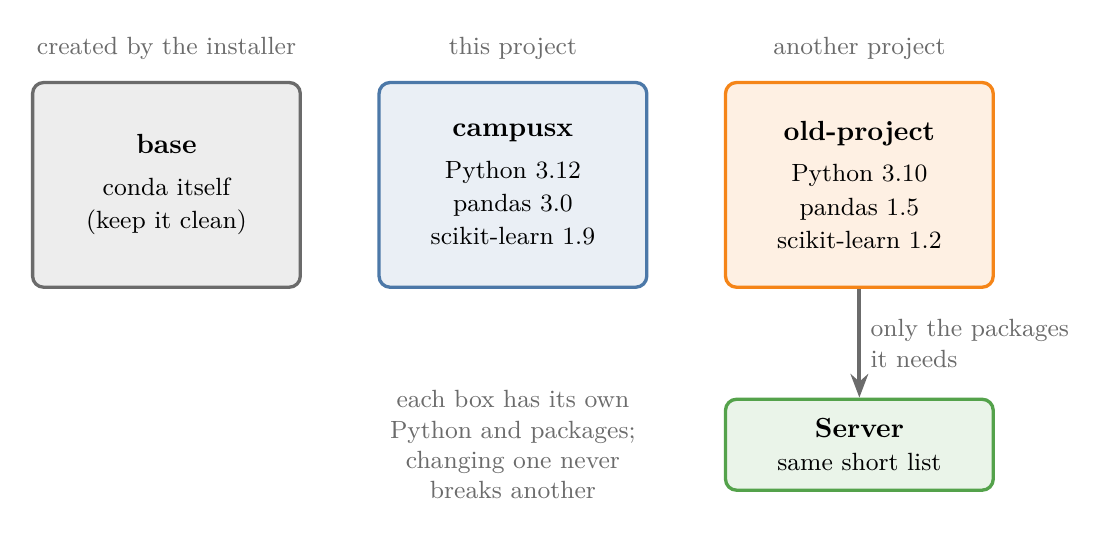
\begin{tikzpicture}
  \node[box=cgrey, minimum width=3.4cm, minimum height=2.6cm] (base) at (0,0)
    {\textbf{base}\\[3pt]{\small conda itself}\\{\small (keep it clean)}};
  \node[box=cblue, minimum width=3.4cm, minimum height=2.6cm] (cx) at (4.4,0)
    {\textbf{campusx}\\[3pt]{\small Python 3.12}\\{\small pandas 3.0}\\{\small scikit-learn 1.9}};
  \node[box=corange, minimum width=3.4cm, minimum height=2.6cm] (old) at (8.8,0)
    {\textbf{old-project}\\[3pt]{\small Python 3.10}\\{\small pandas 1.5}\\{\small scikit-learn 1.2}};
  \node[note, above=4pt of base] {created by the installer};
  \node[note, above=4pt of cx] {this project};
  \node[note, above=4pt of old] {another project};
  \node[box=cgreen, minimum width=3.4cm] (srv) at (8.8,-3.3) {\textbf{Server}\\{\small same short list}};
  \draw[arrow] (old) -- node[note, right, align=left] {only the packages\\it needs} (srv);
  \node[note] at (4.4,-3.3) {each box has its own\\Python and packages;\\changing one never\\breaks another};
\end{tikzpicture}
\end{document}
